The calendar-based rule identifies 1,944 low-history POIs and 299,376 December test events, of which 53,212 (\(17.8\%\)) have positive visits.
The zero forecast has a low-history MAE of \(0.224\), despite recovering no positive visits.
In Table~\ref{tab:zero_collapse_diagnostic}, Fixed-MTGNN with identity adjacency has lower low-history MAE than GraphGRU, \(0.242\) versus \(0.253\), but also lower DMR, \(7.9\%\) versus \(12.0\%\).
NLinear-ridge and TSB recover more positive visit mass, with DMR of \(23.4\%\) and \(27.5\%\), while activating more zero-visit events.
Thus, the ordering by MAE differs from the ordering by positive-visit recovery.

\begin{table}[!htbp]
\centering
\begingroup
\singlespacing
\fontsize{9pt}{10.5pt}\selectfont
\setlength{\tabcolsep}{4pt}
\renewcommand{\arraystretch}{1.08}
\caption{December forecasting diagnostics at $T=14$, $H=7$. The low-history cohort contains the same 1,944 POIs in every row. DMR, FAR, recall, and AP are percentages; activation uses 0.5 visits.}
\label{tab:zero_collapse_diagnostic}
\begin{adjustbox}{max width=\linewidth}
\begin{tabular}{lrrrrrr}
\toprule
Model / adjacency & All MAE & Low-history MAE & DMR & FAR & Recall & AP \\
\midrule
Zero forecast & 2.411 & 0.224 & 0.0 & 0.0 & 0.0 & 17.8 \\
Historical average & 1.483 & 0.336 & 19.2 & 0.3 & 0.7 & 25.5 \\
NLinear-ridge & 1.273 & 0.301 & 23.4 & 9.2 & 21.0 & 26.8 \\
TSB & 1.337 & 0.334 & 27.5 & 8.9 & 21.9 & 29.2 \\
Shared-LSTM & $1.360\pm 0.013$ & $0.251\pm 0.008$ & $12.0\pm 1.5$ & $1.8\pm 0.2$ & $7.0\pm 0.8$ & $28.0\pm 0.5$ \\
GraphGRU, Identity & $1.302\pm 0.007$ & $0.253\pm 0.007$ & $12.0\pm 1.2$ & $2.2\pm 0.4$ & $7.8\pm 0.9$ & $26.4\pm 0.3$ \\
GraphGRU, NAICS-2 & $1.336\pm 0.007$ & $0.267\pm 0.011$ & $11.7\pm 2.1$ & $4.6\pm 1.1$ & $9.4\pm 2.0$ & $21.6\pm 0.5$ \\
GraphGRU, NAICS-4 & $1.350\pm 0.004$ & $0.261\pm 0.009$ & $11.0\pm 2.1$ & $3.4\pm 0.9$ & $7.9\pm 1.9$ & $21.9\pm 0.5$ \\
Fixed-MTGNN, Identity & $1.227\pm 0.005$ & $0.242\pm 0.011$ & $7.9\pm 1.9$ & $1.0\pm 0.2$ & $4.4\pm 0.8$ & $26.1\pm 0.6$ \\
Fixed-MTGNN, NAICS-2 & $1.222\pm 0.008$ & $0.234\pm 0.008$ & $6.8\pm 1.5$ & $0.9\pm 0.2$ & $4.2\pm 0.7$ & $25.4\pm 0.7$ \\
Fixed-MTGNN, NAICS-4 & $1.222\pm 0.007$ & $0.231\pm 0.006$ & $6.0\pm 1.3$ & $0.8\pm 0.1$ & $3.8\pm 0.5$ & $25.3\pm 1.2$ \\
Adaptive-MTGNN & $1.221\pm 0.007$ & $0.236\pm 0.007$ & $7.4\pm 0.8$ & $1.0\pm 0.1$ & $4.5\pm 0.5$ & $25.9\pm 1.0$ \\
GNN-static & $1.301\pm 0.008$ & $0.245\pm 0.010$ & $10.3\pm 2.3$ & $1.9\pm 0.6$ & $6.9\pm 1.6$ & $25.8\pm 0.9$ \\
\bottomrule
\end{tabular}
\end{adjustbox}
\endgroup
\end{table}


Training loss accounts for a substantial part of this difference.
Table~\ref{tab:calibration_loss} compares the same identity-adjacency architectures under absolute- and squared-error training.
Changing GraphGRU from MAE to MSE raises DMR from \(12.0\%\) to \(23.7\%\), but also raises FAR from \(2.2\%\) to \(7.5\%\) and MAE from \(0.253\) to \(0.328\).
Fixed-MTGNN shows the same shift, with DMR increasing from \(7.9\%\) to \(24.0\%\).
Validation-MAE calibration moves these forecasts toward zero and reduces DMR, showing how minimizing absolute error can favor small forecasts in this cohort.

\begin{table}[!htbp]
\centering
\begingroup
\singlespacing
\fontsize{9pt}{10.5pt}\selectfont
\setlength{\tabcolsep}{4pt}
\renewcommand{\arraystretch}{1.08}
\caption{Loss-function and calibration diagnostics on low-history POIs in December at $T=14$, $H=7$. Neural models use identity adjacency. Calibration minimizes validation MAE. The last two columns use a threshold selected to keep validation FAR at or below 10\%; all rates are percentages.}
\label{tab:calibration_loss}
\begin{adjustbox}{max width=\linewidth}
\begin{tabular}{lrrrrrrr}
\toprule
Model (training loss) & Raw MAE & Raw DMR & Raw FAR & \makecell{Calibrated\\DMR} & \makecell{Calibrated\\FAR} & \makecell{Matched-threshold\\test FAR} & \makecell{Matched-threshold\\test recall} \\
\midrule
GraphGRU (MAE) & $0.253\pm 0.007$ & $12.0\pm 1.2$ & $2.2\pm 0.4$ & $3.0\pm 1.2$ & $0.3\pm 0.1$ & $13.7\pm 0.2$ & $27.9\pm 0.9$ \\
GraphGRU (MSE) & $0.328\pm 0.029$ & $23.7\pm 3.8$ & $7.5\pm 2.3$ & $1.9\pm 0.8$ & $0.2\pm 0.1$ & $13.5\pm 0.2$ & $27.3\pm 0.7$ \\
Fixed-MTGNN (MAE) & $0.242\pm 0.011$ & $7.9\pm 1.9$ & $1.0\pm 0.2$ & $3.5\pm 0.4$ & $0.4\pm 0.0$ & $13.2\pm 0.3$ & $26.0\pm 1.7$ \\
Fixed-MTGNN (MSE) & $0.353\pm 0.025$ & $24.0\pm 3.4$ & $6.6\pm 5.9$ & $2.0\pm 1.2$ & $0.2\pm 0.1$ & $12.6\pm 0.9$ & $24.0\pm 4.1$ \\
Shared-LSTM (MAE) & $0.251\pm 0.008$ & $12.0\pm 1.5$ & $1.8\pm 0.2$ & $6.5\pm 0.2$ & $0.7\pm 0.0$ & $14.4\pm 0.0$ & $30.6\pm 0.1$ \\
Shared-LSTM (MSE) & $0.273\pm 0.011$ & $16.5\pm 2.0$ & $3.0\pm 0.5$ & $6.4\pm 0.2$ & $0.7\pm 0.0$ & $14.3\pm 0.1$ & $30.2\pm 0.1$ \\
NLinear-ridge & 0.301 & 23.4 & 9.2 & 0.1 & 0.0 & 13.0 & 27.0 \\
TSB & 0.334 & 27.5 & 8.9 & 5.8 & 0.7 & 13.5 & 29.2 \\
\bottomrule
\end{tabular}
\end{adjustbox}
\endgroup
\end{table}


\begin{figure}[!htbp]
\centering
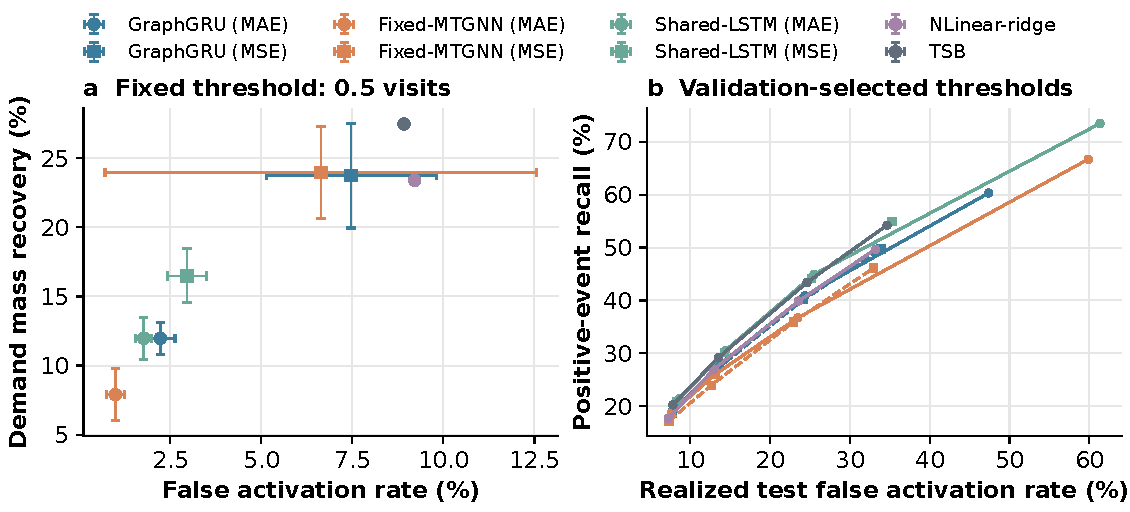
\includegraphics[scale=0.80]{recovery_activation_tradeoff.pdf}
\caption{December diagnostics for the 1,944 low-history POIs at \(T=14\), \(H=7\). Panel (a) shows five-seed means and standard deviations at a fixed 0.5-visit threshold. Panel (b) reports test recall and realized test FAR at thresholds selected for validation FAR targets of \(5\%,10\%,20\%,30\%\).}
\label{fig:recovery_activation_tradeoff}
\end{figure}

Threshold matching gives a different comparison from forecast magnitude alone.
At the \(10\%\) validation-FAR target, GraphGRU trained with MAE attains \(27.9\%\) December recall, compared with \(30.6\%\) for Shared-LSTM and \(29.2\%\) for TSB; their realized test FARs are \(13.7\%\), \(14.4\%\), and \(13.5\%\), respectively.
GraphGRU trained with MSE has similar matched-threshold recall of \(27.3\%\), despite its much larger raw DMR.
Figure~\ref{fig:recovery_activation_tradeoff} shows this distinction across the four validation targets.
With the same fitted models and thresholds in January, recall is \(39.3\%\) for MAE-trained GraphGRU, \(42.7\%\) for Shared-LSTM, and \(41.2\%\) for TSB, at realized FARs of \(14.6\%\), \(15.8\%\), and \(14.7\%\).
Forecast magnitude and matched-threshold detection describe different aspects of intermittent-visit recovery; Shared-LSTM and TSB achieve higher matched-threshold recall than GraphGRU in these comparisons.

\begin{table}[!htbp]
\centering
\begingroup
\singlespacing
\fontsize{9pt}{10.5pt}\selectfont
\setlength{\tabcolsep}{4pt}
\renewcommand{\arraystretch}{1.08}
\caption{January diagnostics for the fixed low-history cohort at $T=14$, $H=7$. Models, calibration, and activation thresholds retain their original validation choices. All rates are percentages.}
\label{tab:january_low_history}
\begin{adjustbox}{max width=\linewidth}
\begin{tabular}{lrrrrrr}
\toprule
Model (training loss) & MAE & DMR & FAR & AP & Matched test FAR & Matched test recall \\
\midrule
GraphGRU (MAE) & $0.331\pm 0.006$ & $27.7\pm 0.9$ & $3.2\pm 0.4$ & $41.6\pm 0.3$ & $14.6\pm 0.3$ & $39.3\pm 0.9$ \\
GraphGRU (MSE) & $0.395\pm 0.026$ & $38.0\pm 2.8$ & $8.5\pm 2.3$ & $42.9\pm 0.5$ & $14.3\pm 0.3$ & $38.7\pm 0.8$ \\
Fixed-MTGNN (MAE) & $0.323\pm 0.010$ & $23.4\pm 1.5$ & $1.7\pm 0.3$ & $42.1\pm 0.7$ & $14.1\pm 0.4$ & $38.1\pm 1.6$ \\
Fixed-MTGNN (MSE) & $0.422\pm 0.021$ & $35.9\pm 2.8$ & $7.7\pm 5.8$ & $41.9\pm 1.3$ & $13.4\pm 1.0$ & $35.0\pm 4.4$ \\
Shared-LSTM (MAE) & $0.332\pm 0.006$ & $26.9\pm 1.3$ & $2.8\pm 0.3$ & $43.3\pm 0.7$ & $15.8\pm 0.1$ & $42.7\pm 0.1$ \\
Shared-LSTM (MSE) & $0.349\pm 0.010$ & $31.5\pm 1.6$ & $4.2\pm 0.6$ & $44.3\pm 0.3$ & $15.5\pm 0.1$ & $42.2\pm 0.1$ \\
NLinear-ridge & 0.368 & 39.4 & 9.7 & 42.5 & 13.3 & 37.9 \\
TSB & 0.402 & 41.3 & 10.2 & 45.0 & 14.7 & 41.2 \\
\bottomrule
\end{tabular}
\end{adjustbox}
\endgroup
\end{table}

